%%%%%%%%%%%%%%%%%%%%%%%%%%%%%%%%%%%%%%%%%%%%%%%
\chapter{Frame Error Rate for AWGN Channel}
 \label{chap:AWGN chain}
%%%%%%%%%%%%%%%%%%%%%%%%%%%%%%%%%%%%%%%%%%%%%%%
\graphicspath{{C:/Users/Kevin/Bachelarbeit/Bachelorarbeit/01_Bachelorarbeit_LaTex/02_Figures/}}

This section will further built upon the topics discussed in the previous chapters. We will now build a communication chain using the blocks discussed in Chapter 2. After the transmission the \gls{FER} will be determined. The \gls{FER}\footnote{FER = $\frac{\textrm{Number of faulty frames in a simulation}}{\textrm{Number of all frames in a simulation}}$} is the estimated rate of faulty transmissions in one whole simulation. We will be sending frames of code words each consisting of 576 up to 2048 bits. After comparison between the sent code word and the decoded code word at the receiver we determine a frame error. If the decoded codeword has any wrong bit the whole frame will be marked as a faulty frame. This will be done for a certain amount of frames.

\section{LDPC and the Coded Modulation Library}
Already explained in Chapter 1 the whole transmission will be done with the coding method of \gls{LDPC}. For the coding and decoding we will be using the Coded Modulation Library. This library and the functions used in this simulation will be further explained now.
\newline
The Iterative Solutions Coded Modulation Library (ISCML) is an open source toolbox for simulating capacity approaching codes in MATLAB\cite{CML}. The toolbox supports many different standard linear block codes and turbo codes. With many of the complex and computational heavy codes implemented in C and ported back to MATLAB as so called C-mex functions\cite{CML}.
\newline 
For this thesis a further look will be taken at the WiMax LDPC code. The coder function will create the parity-check-matrix \textbf{H} with a given codeword length $n$, message length $k$ and rate $r$. The code word which will be sent will be created like this:
\begin{equation}
\label{eq:LDPC1}
\boldmath c = m\mathbf{G},
\end{equation}
with $c$ being the code word transmitted, $m$ the message send and $\mathbf{G}$ the generator matrix used. The generator matrix $\mathbf{G}$ is defined as follows:
\begin{equation}
\label{eq:generator}
\boldmath{G} = [\mathbf{I}_k|\mathbf{P}],
\end{equation}
where $\mathbf{I}_k$ is the $k \times k$ identity matrix and $\mathbf{P}$ the matrix $k \times (n-k)$.
Out of the generator matrix $\mathbf{G}$ the check parity matrix can be computed:
\begin{equation}
\label{eq:CHPAR}
\mathbf{H} = [-\mathbf{P}^T|I_{n-k}],
\end{equation}
%\begin{equation}
%\label{eq:LDPC2}
%a_r = (\mathbf{H}_k)^{-1} * H_l * a_n
%\end{equation}
The decoding will also be done by the \gls{CML} which again uses the parity-check matrix \textbf{H}. The received code word has to fulfill this condition:
\begin{equation}
\label{eq:LDPC3}
\boldmath{H}*b^T = 0,
\end{equation}
with $b^T$ being the received code word. This will be checked with typical graph solving algorithms. For LDPC the commonly used algorithm is the sum-product algorithm.
With the \gls{CML} the first and last block of the full communication chain (\fig{fig:commchain}) is implemented.
\section{Demapping after AWGN}
Another big part of a functioning communication chain is the estimation of the code word from the received symbol stream $\boldmath\underline{Y}$, which passed the channel experiencing various kind of noises and fadings. There are two main forms of restoring the code word, namely hard-decision demapping and soft-decision demapping.
\subsection{Hard-Decision Demapping vs. Soft-Decision Demapping}
We will now discuss the benefits between hard-decision and soft-decision demapping. Hard-decision demapping makes a decision based on the decision boundary of the received symbol. While soft demapping will take into consideration all symbol constellations in the modulation scheme. For soft demapping a reliability of the decision can be given by computing the euclidean distance to every constellation symbol.
It is proven that soft demapping will achieve better demapping results while hard demapping is not as complex as soft demapping \cite{GaussianWaves}.In our case we do not mind a more complex system which takes more time but are more focused on achieving the maximum rate of successful transmissions.
\newpage
\subsection{Log-Likelihood Ratio}
A soft demapper will now be implemented in this system. The soft demapper will result in turning the symbols in the corresponding bit block.
\begin{figure}[!htb]
    \centering
    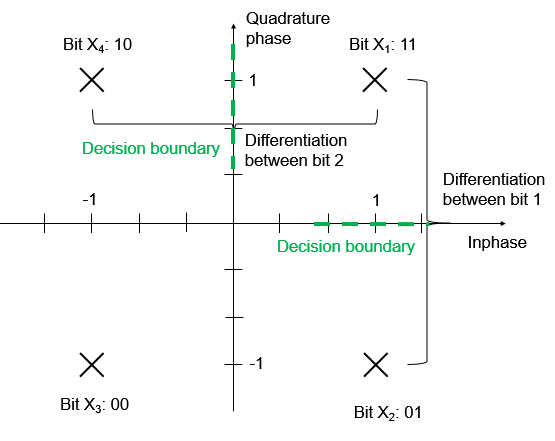
\includegraphics[width=0.8\textwidth]{llr.png}
    \caption{Depiction of soft demapper in I/Q-plane}
    \label{fig:llr}
\end{figure}
\newline
As seen in the figure above we have a \gls{QPSK} modulated codeword. Symbols \textbf{\underline{Y}} received can be located anywhere on the I/Q-plane distorted by AWGN. We will now assume a single symbol $Y$ received at the demapper.
With QPSK consisting of two bit blocks $[B_1B_2]$ first a differentiation for the first bit is done.
\begin{equation}
\label{eq:llr1}
L = log\frac{P(B_1=0|Y)}{P(B_1=1|Y)}
\end{equation}
With Baye's rule:
\begin{equation}
\label{eq:bl}
P(B_1=0|Y) = \frac{P(Y|B_1=0)}{p(Y)}*P(B_1=0),
\end{equation}
the equation simplifies to 
\begin{equation}
L = log\frac{P(Y|B_1=0)}{P(Y|B_1=1)},
\end{equation}
with $P(B1=0)=P(B1=1)=0.5$.
Getting back to \fig{fig:llr} it can be determined that $X_1$ and $X_4$ have $B_1=1$ while $X_2$ and $X_3$ result in $B_1=0$.
\begin{equation}
L = log\frac{P(Y|X_2)+P(Y|X_3)}{P(Y|X_1)+P(Y|X_4)}.
\end{equation}
With \eq{eq:AWGNpdf} the log likelihood for bit $B_1$ can now be calculated. The corresponding bit $B_2$ will also be determined analogous. In the end a code word is received as log likelihood ratios and provided to the channel decoder \cite{SoftDemapping}.
\section{FER}
\label{sec:FER}
The \gls{FER} can now be determined with the help of the two previous sections. By dividing the number of faulty frames from the total number of frames we get the \gls{FER}. It should be noted that not every \gls{FER} calculated is a reliable result for our simulation. For a whole simulation run a certain amount of faulty frames is needed, usually at least 50 faulty frames need to be detected. It can be seen like this: A simulation run for 100 frames with 1 faulty frame does not give a confident result of a \gls{FER} of 0.01. While a simulation ran for 10000 frames with 100 faulty frames will be seen as a more reliable result for a \gls{FER} of 0.01. 
\newline
With the proposition above for a \gls{FER} of $10^{-4}$ we would need to run a simulation with $10^6$ frames. Now the problem of simulation time length arises. If lower \gls{FER} needs to be calculated the number of frames will rise. Also while maybe feasible for short SNR ranges some calculations will need longer SNR-ranges, which becomes a problem in the further chapters for fading channels. Both combined will make the simulation run rather long.
\newline
Two methods to reduce the simulation time are now implemented: The first one being a premature break of the simulation after reaching 100 faulty frames and dividing by the number of iterations ran.
\begin{equation}
\textrm{FER} = \frac{100}{\textrm{Number of frames run so far in the simulation}}
\end{equation}
Even if running the whole simulation resulting in more precise \gls{FER}, 100 faulty frames are enough for plotting a reliable result. Another technique is to increase the step size of the SNR between simulations, which will allow us to keep the SNR range at the expense of plot resolution. This can be mitigated by interpolating the results, which means we numerically create more data samples to increase the plot resolution.

\newpage
\section{Simulation Results}
All the above discussed methods are implemented in MATLAB.
The simulation will be run for an SNR range of 0\,dB-10\,dB SNR. Furthermore a \gls{FER} of at least $10^{-3}$ should be calculated, which is a total of 10000 frames run. The \gls{FER} can be plotted over the corresponding \gls{SNR} seen in \fig{fig:FERAWGN}.  
\newline
Setting a threshold at a \gls{FER} of $10^{-3}$, that means when the function reaches the desired value, the corresponding \gls{SNR} value is noted down. The value is then plotted into the capacity plot (\fig{fig:capmod}) from Chapter \ref{chap:awgnchan}. It has to be taken into account the rate of \gls{LDPC} coding used. The rate defines the amount of relevant data in a whole frame/code word. That means for a rate of $1/2$ the transmission of relevant data is halved. For QPSK with a maximum of 2 bits per symbols and a rate of $1/2$ information value of only 1 bit per symbol can be achieved.
\newline
\begin{figure}[!htb]
	\setlength\fwidth{0.9\textwidth}
	\setlength\fheight{0.4\textheight}
	\centering
	% This file was created by matlab2tikz.
%
%The latest updates can be retrieved from
%  http://www.mathworks.com/matlabcentral/fileexchange/22022-matlab2tikz-matlab2tikz
%where you can also make suggestions and rate matlab2tikz.
%
\definecolor{mycolor1}{rgb}{0.00000,0.44700,0.74100}%
\definecolor{mycolor2}{rgb}{0.74902,0.00000,0.74902}%
\definecolor{mycolor3}{rgb}{0.85098,0.32549,0.09804}%
\definecolor{mycolor4}{rgb}{0.46667,0.67451,0.18824}%
%
\begin{tikzpicture}

\begin{axis}[%
width=0.951\fwidth,
height=\fheight,
at={(0\fwidth,0\fheight)},
scale only axis,
xmin=-5,
xmax=25,
xlabel style={font=\color{white!15!black}},
xlabel={SNR in dB},
ymin=0,
ymax=2.5,
ylabel style={font=\color{white!15!black}},
ylabel={Bits per symbol},
axis background/.style={fill=white},
title style={font=\bfseries},
title={FER (0.001) of QPSK with Gaussian Noise},
xmajorgrids,
ymajorgrids,
legend style={at={(0.05,0.65)}, anchor=south west, legend cell align=left, align=left, draw=white!15!black}
]
\addplot [color=mycolor1, line width=1.5pt]
  table[row sep=crcr]{%
-6	0.323068206330696\\
-5	0.391326071720055\\
-4	0.48489476841884\\
-3	0.574809791357794\\
-2	0.698200176432383\\
-1	0.833818491736498\\
0	0.972778527481442\\
1	1.12495846691126\\
2	1.28072065748154\\
3	1.44250305591488\\
4	1.58596017892716\\
5	1.722479934533\\
6	1.82567644583971\\
7	1.89431417542903\\
8	1.95776065265052\\
9	1.98017610381626\\
10	1.99433936158288\\
11	1.99258273944893\\
12	2.00345231173243\\
13	1.99904308404509\\
14	1.99922794452327\\
15	2.00370158206796\\
16	2.00276837542221\\
17	1.99652877120277\\
18	1.99843303166521\\
19	1.9989850606081\\
20	2.00488508312673\\
21	1.98995611336795\\
22	2.00455104085159\\
23	1.99686202453218\\
24	1.99923283598126\\
25	1.99341493446232\\
26	2.00059528376659\\
};
\addlegendentry{QPSK}

\addplot [color=blue, draw=none, mark size=5.0pt, line width = 1.0pt, mark=asterisk, mark options={solid, blue}]
  table[row sep=crcr]{%
1.9841	1\\
};
\addlegendentry{R = 1/2}

\addplot [color=mycolor2, draw=none, mark size=5.0pt, line width = 1.0pt, mark=asterisk, mark options={solid, mycolor2}]
  table[row sep=crcr]{%
3.9409	1.33333333333333\\
};
\addlegendentry{R = 2/3}
\addplot [color=mycolor3, draw=none, mark size=5.0pt, line width = 1.0pt, mark=asterisk, mark options={solid, mycolor3}]
  table[row sep=crcr]{%
4.9859	1.5\\
};
\addlegendentry{R = 3/4}
\addplot [color=mycolor4, draw=none, mark size=5.0pt, line width = 1.0pt, mark=asterisk, mark options={solid, mycolor4}]
  table[row sep=crcr]{%
5.991	1.66666666666667\\
};
\addlegendentry{R = 5/6}
\end{axis}
\end{tikzpicture}%
	\caption{Capacity and TX/RX-chain simulation for QPSK. Plotted points correspond FER of $10^{-3}$}
	\label{fig:llr1}
\end{figure}
\begin{figure}[!htb]
	\setlength\fwidth{0.9\textwidth}
	\setlength\fheight{0.4\textheight}	
	\centering
	% This file was created by matlab2tikz.
%
%The latest updates can be retrieved from
%  http://www.mathworks.com/matlabcentral/fileexchange/22022-matlab2tikz-matlab2tikz
%where you can also make suggestions and rate matlab2tikz.
%
\definecolor{mycolor1}{rgb}{0.00000,0.44700,0.74100}%
\definecolor{mycolor2}{rgb}{0.74902,0.00000,0.74902}%
\definecolor{mycolor3}{rgb}{0.85098,0.32549,0.09804}%
\definecolor{mycolor4}{rgb}{0.00000,0.49804,0.00000}%
%
\begin{tikzpicture}

\begin{axis}[%
width=0.951\fwidth,
height=\fheight,
at={(0\fwidth,0\fheight)},
scale only axis,
xmin=-5,
xmax=25,
xlabel style={font=\color{white!15!black}},
xlabel={SNR in dB},
ymin=0,
ymax=4.5,
ylabel style={font=\color{white!15!black}},
ylabel={Bits per symbol},
axis background/.style={fill=white},
title style={font=\bfseries},
title={FER (0.001) of QAM16 with Gaussian Noise},
xmajorgrids,
ymajorgrids,
legend style={at={(0.1,0.55)}, anchor=south west, legend cell align=left, align=left, draw=white!15!black}
]
\addplot [color=mycolor1, line width=1.5pt]
  table[row sep=crcr]{%
-6	0.328621714082722\\
-5	0.410274595889064\\
-4	0.497750186881902\\
-3	0.599712705644915\\
-2	0.714042374792633\\
-1	0.861837472466473\\
0	1.00371041314962\\
1	1.17925231331639\\
2	1.36317896763643\\
3	1.56645355738085\\
5	1.9914221739593\\
6	2.22277316719511\\
7	2.45551845122164\\
8	2.70357747937736\\
9	2.93827693641367\\
10	3.18009610376135\\
11	3.38994681065897\\
12	3.57915476353915\\
13	3.73698103166151\\
14	3.85191363323502\\
15	3.93083271031978\\
16	3.98124687547666\\
17	3.98873587025561\\
18	3.9999092584337\\
19	3.99126898886324\\
20	4.00461627105919\\
22	3.99570005449973\\
23	4.00385440769931\\
24	3.99872083361317\\
25	4.0013615285833\\
26	3.99772619520965\\
};
\addlegendentry{QAM-16}

\addplot [color=blue, draw=none, mark size=5.0pt, line width = 1.0pt, mark=asterisk, mark options={solid, blue}]
  table[row sep=crcr]{%
8.4925	2\\
};
\addlegendentry{R = 1/2}

\addplot [color=mycolor2, draw=none, mark size=5.0pt, line width = 1.0pt, mark=asterisk, mark options={solid, mycolor2}]
  table[row sep=crcr]{%
10.94	2.66666666666667\\
};
\addlegendentry{R = 2/3}

\addplot [color=mycolor3, draw=none, mark size=5.0pt, line width = 1.0pt, mark=asterisk, mark options={solid, mycolor3}]
  table[row sep=crcr]{%
11.9828	3\\
};
\addlegendentry{R = 3/4}

\addplot [color=mycolor4, draw=none, mark size=5.0pt, line width = 1.0pt, mark=asterisk, mark options={solid, mycolor4}]
  table[row sep=crcr]{%
12.9956	3.33333333333333\\
};
\addlegendentry{R = 5/6}

\end{axis}
\end{tikzpicture}%
	\caption{Capacity and TX/RX-chain simulation for 16-QAM. Plotted points correspond FER of $10^{-3}$}
	\label{fig:llr2}
\end{figure}
\begin{figure}[!h]
	\setlength\fwidth{0.9\textwidth}
	\setlength\fheight{0.4\textheight}
	\centering
	% This file was created by matlab2tikz.
%
%The latest updates can be retrieved from
%  http://www.mathworks.com/matlabcentral/fileexchange/22022-matlab2tikz-matlab2tikz
%where you can also make suggestions and rate matlab2tikz.
%
\definecolor{mycolor1}{rgb}{0.00000,0.44700,0.74100}%
\definecolor{mycolor2}{rgb}{0.74902,0.00000,0.74902}%
\definecolor{mycolor3}{rgb}{0.85098,0.32549,0.09804}%
\definecolor{mycolor4}{rgb}{0.46667,0.67451,0.18824}%
%
\begin{tikzpicture}

\begin{axis}[%
width=0.951\fwidth,
height=\fheight,
at={(0\fwidth,0\fheight)},
scale only axis,
xmin=0,
xmax=30,
xlabel style={font=\color{white!15!black}},
xlabel={SNR in dB},
ymin=0,
ymax=6.5,
ylabel style={font=\color{white!15!black}},
ylabel={Bits per symbol},
axis background/.style={fill=white},
title style={font=\bfseries},
title={FER (0.001) of QAM64 with Gaussian Noise},
xmajorgrids,
ymajorgrids,
legend style={at={(0.1,0.55)}, anchor=south west, legend cell align=left, align=left, draw=white!15!black}
]
\addplot [color=mycolor1, line width=1.5pt]
  table[row sep=crcr]{%
-1	0.83078278973122\\
0	0.979654599592624\\
1	1.14834131414807\\
2	1.33127288676911\\
4	1.74508866458763\\
5	1.96566337984369\\
6	2.21403226346695\\
7	2.45940311575263\\
8	2.71491729771481\\
10	3.24616258413947\\
13	4.09660026502285\\
14	4.38419050112642\\
15	4.67504652219285\\
16	4.95776784876414\\
17	5.22003469749198\\
18	5.45597897518436\\
19	5.65235382550127\\
20	5.79883674591287\\
21	5.89932124254842\\
22	5.95960529647478\\
23	5.98793504239796\\
24	5.99162626739952\\
25	6.00358017470219\\
26	5.99555782274282\\
27	5.99166132276335\\
28	5.99097580881566\\
29	6.00114495777247\\
30	5.98912057361096\\
31	6.00260416766955\\
};
\addlegendentry{QAM-64}

\addplot [color=blue, draw=none, mark size=5.0pt, line width = 1.0pt, mark=asterisk, mark options={solid, blue}]
  table[row sep=crcr]{%
14.4588	3\\
};
\addlegendentry{R = 1/2}

\addplot [color=mycolor2, draw=none, mark size=5.0pt, line width = 1.0pt, mark=asterisk, mark options={solid, mycolor2}]
  table[row sep=crcr]{%
16.9043	4\\
};
\addlegendentry{R = 2/3}

\addplot [color=mycolor3, draw=none, mark size=5.0pt, line width = 1.0pt, mark=asterisk, mark options={solid, mycolor3}]
  table[row sep=crcr]{%
17.9863	4.5\\
};
\addlegendentry{R = 3/4}

\addplot [color=mycolor4, draw=none, mark size=5.0pt, line width = 1.0pt, mark=asterisk, mark options={solid, mycolor4}]
  table[row sep=crcr]{%
19.3035	5\\
};
\addlegendentry{R = 5/6}

\end{axis}
\end{tikzpicture}%
	\caption{Capacity and TX/RX-chain simulation for 64-QAM. Plotted points correspond FER of $10^{-3}$}
	\label{fig:llr3}
\end{figure}

\newpage
The first \fig{fig:llr1} shows the QPSK capacity plot from \fig{fig:capmod}. The capacity plot is needed to give reference for the \gls{FER} points. For any \gls{FER} point found it needs to be close to the capacity plot but not surpass or even closely approach the plot. It can be seen that for all four rates simulated the points are not surpassing the \gls{SNR}, and therefore the efficiency of the initial  capacity plot.
For the next two figures, \fig{fig:llr2} and \fig{fig:llr3}, the same procedure has been done. For all four available rates in WiMax coding the corresponding SNR value for the \gls{FER} of $10^{-3}$ is plotted. It can be observed that also for these plots every rate is below the corresponding calculated capacity plot. 
\newline
Next we compare the overall transmission power difference between the optimal capacity achievable and the simulated BICM system. For this the before plotted \gls{FER} are compared to the capacity plot. The \gls{SNR} difference between these two, to achieve the same bits per symbol rate, can be read out of the figures. 
In \fig{fig:llr1} to reach the \gls{FER} for the rate of $1/2$ from the capacity plot an increase of about 2\,dB is needed. This corresponds to a increase of the factor 1.6 in terms of power\footnote{$\textrm{SNR in W} = 10^{\frac{SNR\_dB}{10}}$} needed to reach the \gls{FER} of 0.001. The same observation done for both 16-QAM and 64-QAM will result in deviating results. For 16-QAM an increase of about 3\,dB is needed, which corresponds to an increase of power of the factor 2. 64-QAM on the other hand needs about 5\,dB, which results into a overall increase of power consumption of the factor 3.
\newline
Another observation from all three plots is the decrease in \gls{SNR} needed for higher rates. While not very significant for \gls{QPSK} where the decrease for the rate $1/2$ to $5/6$ is not very noticeable, the decrease in the other two plots is remarkable. For 16-QAM we save about 1\,dB and for 64-QAM the save is 2\,dB.
In general it is to be expected that a simulation for a real communication chain is outperformed by the theoretical calculations done in Chapter 3. With the comparison between the \gls{FER} points and the previous calculated capacity plots the simulation for a working transmitter receiver is confirmed and can be used for further simulations with different channel settings.




